
%dash pattern=on 5pt off 2pt
%[fill = white, rounded corners = 4pt, inner sep = 1pt]
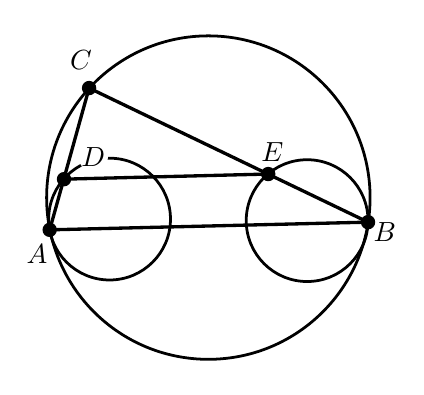
\begin{tikzpicture}[scale = 0.65]
    \clip(12.22,3.3) rectangle (19.42,9.93);
    \draw [line width=1pt] (13.82,6.19) circle (1.19cm);
    \draw [line width=1pt] (17.68,6.16) circle (1.19cm);
    \draw [line width=1pt] (15.75,6.61) circle (3.16cm);
    \draw [line width=1.2pt] (12.65,5.98)-- (18.87,6.13);
    \draw [line width=1.2pt] (18.87,6.13)-- (13.42,8.75);
    \draw [line width=1.2pt] (13.42,8.75)-- (12.65,5.98);
    \draw [line width=1.2pt] (12.93,6.97)-- (16.92,7.07);
    \begin{scriptsize}
        \normalsize
        \fill [color=black] (12.65,5.98) circle (4pt);
        \draw[color=black] (12.4,5.5) node[fill = white, rounded corners = 4pt, inner sep = 1pt] {$A$};
        \fill [color=black] (18.87,6.13) circle (4.0pt);
        \draw[color=black] (19.2,5.93) node {$B$};
        \fill [color=black] (12.93,6.97) circle (4.0pt);
        \draw[color=black] (13.5,7.4) node[fill = white, rounded corners = 4pt, inner sep = 1pt] {$D$};
        \fill [color=black] (16.92,7.07) circle (4.0pt);
        \draw[color=black] (17,7.5) node[fill = white, rounded corners = 4pt, inner sep = 1pt] {$E$};
        \fill [color=black] (13.42,8.75) circle (4.0pt);
        \draw[color=black] (13.26,9.3) node[fill = white, rounded corners = 4pt, inner sep = 1pt] {$C$};
    \end{scriptsize}
\end{tikzpicture}